
\begin{figure}
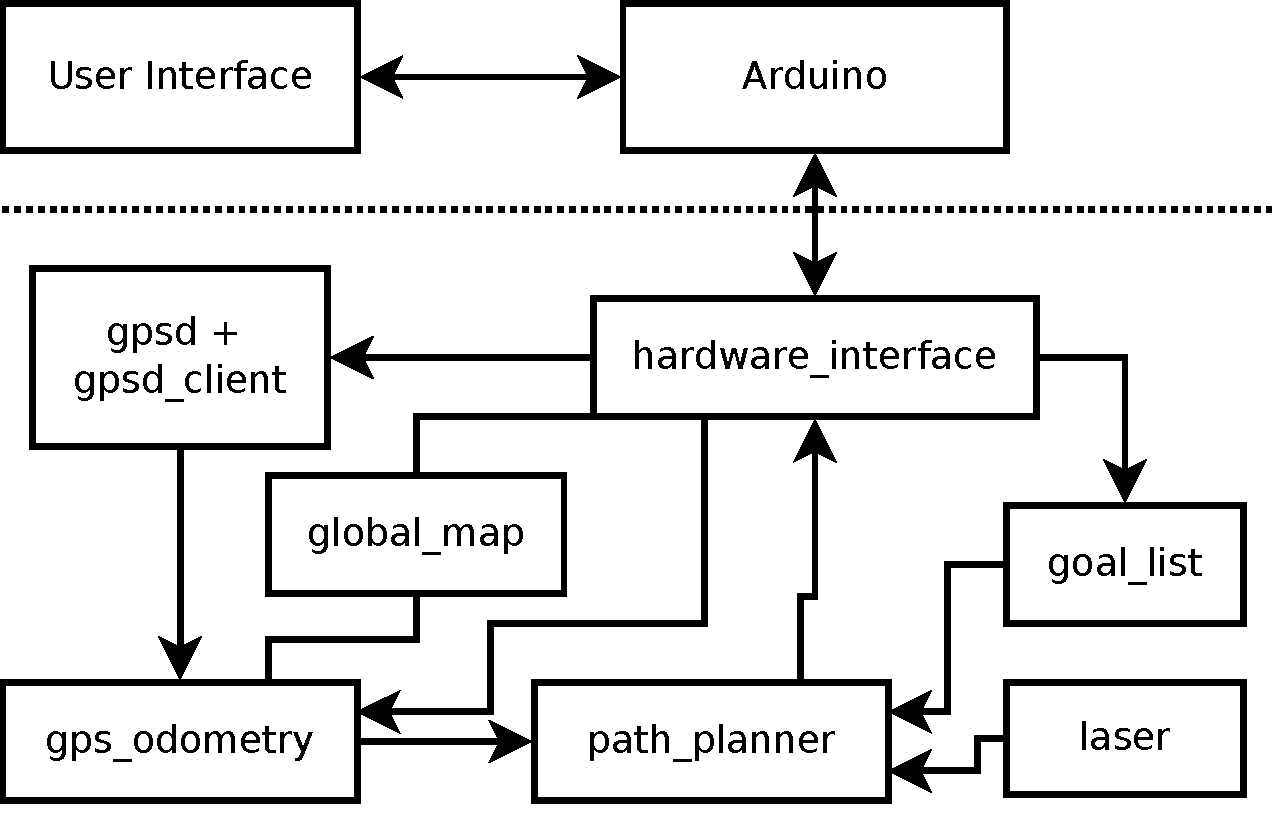
\includegraphics[width=1\textwidth]{software_flow}
\caption{Software Architecture}
\end{figure}

The primary computer runs Gentoo, a Linux distribution, and runs the ROS software package to support the high-level behaviors. Each behavior or part of the system is implemented as a separate ROS node, and communicates with other nodes through messages or service calls.

There wasn't enough time to implement all of the ROS nodes in the original design before the Sparkfun AVC, so a subset of these modules were implemented. In particular, there wasn't enough time to write the localization or active localization nodes, and problems with the path planner resulted in it being replaced by a reactive goal tracking and obstacle avoidance algorithm.

The hardware\_interface node is responsible for translating data from the Arduino into ROS messages, and for translating some ROS messages into control and status data to be sent to the Arduino. 

The hardware\_interface node recieves odometry, bump sensor, battery level, GPS, and compass data from the Arduino. It translates the odometry data into odometry messages, using a kinematic model of the robot to translate encoder counts and wheel movements into position change in x, y, and heading. It translates the compass data (really an x-y magnetometer) into a heading from north, and publishes that angle in a compass message. It takes the GPS data, as NMEA strings, and sends it to an instance of gpsd\cite{gpsd}, which parses the data, and publishes it, to be read by the gpsd\_client node, which publishes the resulting data as GPSFix messages. It records the battey level data into a log file, for later analysis; eventually, this data will be used to build a model to predict remaining battery capacity. It ignores the bump sensor data. The hardware\_interface node also receives a list of gps coordinates that is forwarded through the Arduino from the user interface, and publishes this as a GoalList message.

The hardware\_interface node recieves command messages as speed and steering commands, and transmits them to the Arduino. It also recieves position estimate messages, translates them into GPS coordinates, and transmits them to the Arduino, to be forwarded to the user interface.

TODO: finish this implementation and report on the results.


